\section{控制实验}

使用设计的凸优化规划-滑膜控制器,在前文提到的柔性支撑支撑Stewart平台的控制上可以进行应用。系统控制框图如图\ref{fig:control_model},根据仿真分析,其满足前面提出的的几个条件:

\begin{enumerate}
    \item 控制器理论上稳定,收敛速度快
    \item 控制器不需要具体动力学模型,参数易调节
    \item 对扰动误差鲁棒性好
    \item 控制器输出相对光滑,频率低,可以直接应用在机械装置上
\end{enumerate}

根据图\ref{fig:kinetic_model}的运动学模型,搭建了实验装置如图\ref{fig:actual_model}所示:

\begin{figure}[H]
    \centering
    \includegraphics[width=0.6\textwidth]{imgs/actual_model.png}
    \caption{实验装置示意图}
    \label{fig:actual_model}
\end{figure}

其中B坐标系被三根绳索悬吊,模拟FAST机构悬浮状态的特点。实验过程中,B受到外力作用发生振动,期望通过控制Stewart平台的6条支链长度来保证C平台在大地坐标系下保持稳定。

B平台的位姿通过6个拉线编码器的长度求得。在特定的构型下,可以很快的得到解析解\cite{williamsCableBasedMetrologySystem2003}。由于本文主要是为了验证提出的算法跟踪效果,因此评价C平台运动的指标是通过支链长度和B平台位姿进行正解求得。如果使用直接测量C在世界坐标系下的位姿,则需要重新标定拉线编码器和Stewart平台的参数,而这和本文主要内容无关。

为了对比实验效果,在实验需求情况下,设计了如下几组实验,如表\ref{tab:experiment}:

\begin{table}[H]
    \small
    \centering
    \caption{实验设计种类}
    \begin{tabular}{lcc}
    \toprule
    控制器类型 & 输入幅值       & 输入频率         \\
    \midrule
    凸优化-自适应滑膜控制器      & 高振幅 40mm &  低频率 0.02Hz \\
    凸优化-自适应滑膜控制器      & 低振幅 15mm &  低频率 0.02Hz \\
    凸优化-自适应滑膜控制器      & 高振幅 40mm &  高频率 0.2Hz \\
    凸优化-自适应滑膜控制器      & 低振幅 15mm &  高频率 0.2Hz \\
    PID控制器      & 高振幅 40mm &  低频率 0.02Hz \\
    PID控制器      & 高振幅 40mm &  高频率 0.2Hz \\
    无控制器      & 高振幅 40mm &  低频率 0.02Hz \\
    无控制器      & 高振幅 40mm &  高频率 0.2Hz \\
    \bottomrule
    \multicolumn{3}{l}{\scriptsize 无控制器指直接将逆解理论值传给支链执行} \\
    \end{tabular}%
    \label{tab:experiment}%
\end{table}%

第一组实验得到的结果如图\ref{fig:C-AH-FL_1_input}-\ref{fig:C-AH-FL_1_c_movement}所示。

\begin{figure}[H]
    \centering
    \subfloat[输入扰动x,y,z三方向振幅]{
    \begin{minipage}[t]{0.4\linewidth}
    \centering
    \includegraphics[width=0.9\textwidth]{imgs/Experiment/C-AH-FL_1_position_B_error.png}
    % \caption{}
    \end{minipage}%
    }%
    \hspace{0.5pt}
    \subfloat[输入扰动RPY角振幅]{
    \begin{minipage}[t]{0.4\linewidth}
    \centering
    \includegraphics[width=0.9\textwidth]{imgs/Experiment/C-AH-FL_1_rpy_B.png}
    % \caption{}
    \end{minipage}%
    }%
    \centering
    \caption[]{凸优化-自适应滑膜控制器对应的输入扰动振幅}
    \label{fig:C-AH-FL_1_input}
\end{figure}

\begin{figure}[H]
    \centering
    \subfloat[6轴实际轴长]{
    \begin{minipage}[t]{0.4\linewidth}
    \centering
    \includegraphics[width=0.9\textwidth]{imgs/Experiment/C-AH-FL_1_axis_actual_length.png}
    % \caption{}
    \end{minipage}%
    }%
    \hspace{0.5pt}
    \subfloat[6轴期望轴长]{
    \begin{minipage}[t]{0.4\linewidth}
    \centering
    \includegraphics[width=0.9\textwidth]{imgs/Experiment/C-AH-FL_1_axis_ideal_length.png}
    % \caption{}
    \end{minipage}%
    }%
    \centering
    \caption[]{凸优化-自适应滑膜控制器在输入高振幅、低频率情况下的轴长响应图}
    \label{fig:C-AH-FL_1_axis}
\end{figure}


\begin{figure}[H]
    \centering
    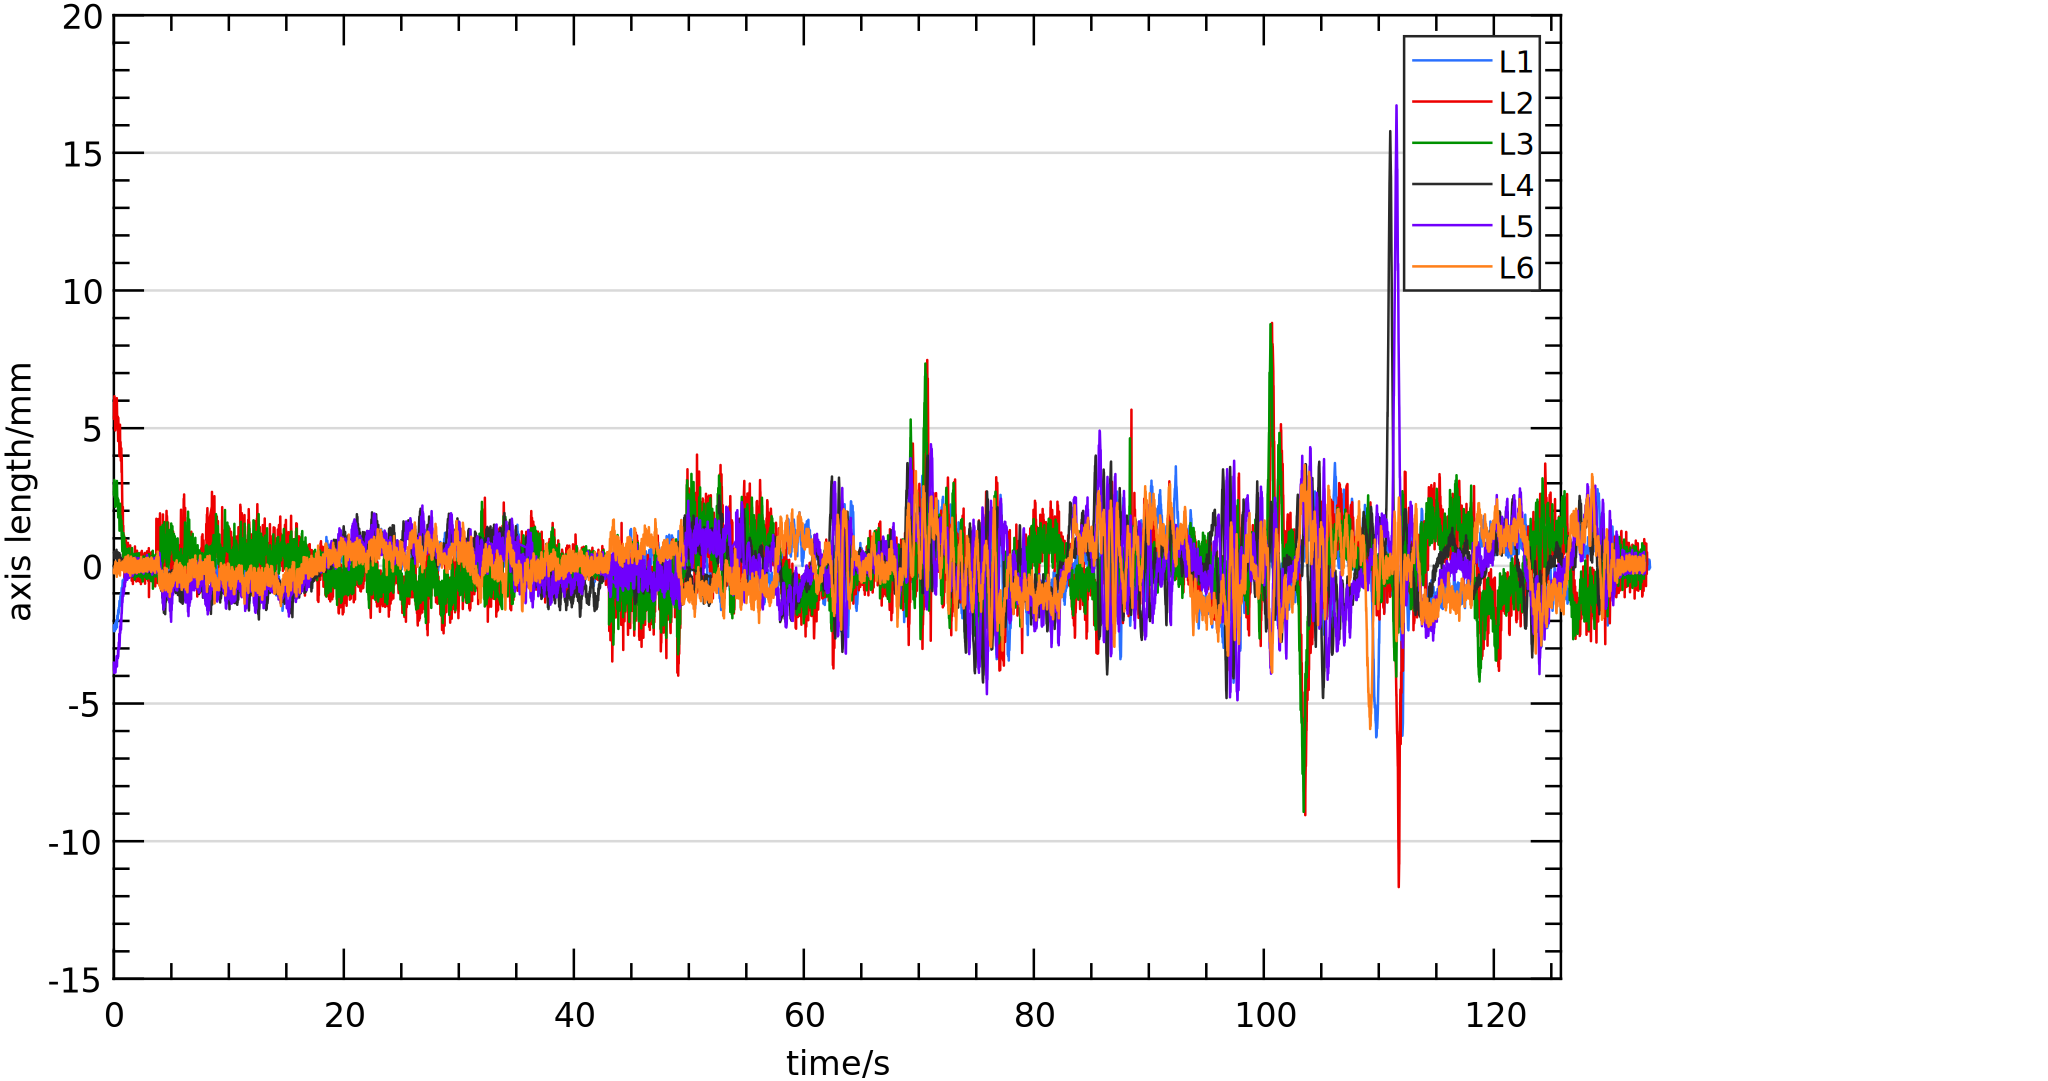
\includegraphics[width=0.6\textwidth]{imgs/Experiment/C-AH-FL_1_axis_diff_length.png}
    \caption{凸优化-自适应滑膜控制器在输入高振幅、低频率情况下的轴长跟踪误差}
    \label{fig:C-AH-FL_1_axis_diff_length}
\end{figure}

\begin{figure}[H]
    \centering
    \includegraphics[width=0.6\textwidth]{imgs/Experiment/C-AH-FL_1_c_movement.png}
    \caption{凸优化-自适应滑膜控制器在输入高振幅、低频率情况下,正解得到的C平台位置移动情况}
    \label{fig:C-AH-FL_1_c_movement}
\end{figure}

在图\ref{fig:C-AH-FL_1_axis_diff_length}中棕色虚线左半边是输入主要为x,y,z三方向对应的幅值变化,右半边的输入则主要是角度变化。可以发现,左半边的抑振效果明显好于右半边,这是因为机构的特性导致的。当机构发生角度偏转时,类似于倒立摆,顶部的C平台的运动会被放大。粗略的计算可以得到,输入角度每变化1度,相当于C平台移动20mm,因此一旦角度变化速度快,凸优化规划器就会限制输出速度,从而导致跟踪误差增大。因此,下面分析输入主要以位置变化的情形为主,角度变化阶段不做考虑。

对每根轴而言,从图\ref{fig:C-AH-FL_1_axis_diff_length}可以看出,其在位置变化阶段基本可以将跟踪误差控制在$\pm 1 \mathrm{mm}$之间,而其变动范围基本为$50 \mathrm{mm}$,即相对的控制精度可以达到$2\%$。从图\ref{fig:C-AH-FL_1_c_movement}可以看出,位置变化情形下,通过本文提出的凸优化-自适应滑膜控制器,可以将C平台每个轴的位置误差控制在$\left[ -5\mathrm{mm},3\mathrm{mm} \right] $左右(其中x轴曲线存在一个$-5\mathrm{mm}$的静偏差,是因为控制开始时的初始位置不同导致的)。

相比输入的幅值条件:x轴$[-40\mathrm{mm}, 50\mathrm{mm}]$,y轴$\left[ -35\mathrm{mm},45\mathrm{mm} \right] $的情况,其幅值范围被抑制到接近$10\%$。对比前文提出的控制要求,这里得到的控制结果优于控制指标。

% todo rms 指标
% \textbf{是否需要计算RMS指标}

对低振幅,高频率的情形,其结果为图\ref{fig:C-AL-FM_1_input}-\ref{fig:C-AL-FM_1_c_movement}:

\begin{figure}[H]
    \centering
    \subfloat[输入扰动x,y,z三方向振幅]{
    \begin{minipage}[t]{0.4\linewidth}
    \centering
    \includegraphics[width=0.9\textwidth]{imgs/Experiment/C-AL-FM_1_position_B_error.png}
    % \caption{}
    \end{minipage}%
    }%
    \hspace{0.5pt}
    \subfloat[输入扰动RPY角振幅]{
    \begin{minipage}[t]{0.4\linewidth}
    \centering
    \includegraphics[width=0.9\textwidth]{imgs/Experiment/C-AL-FM_1_rpy_B.png}
    % \caption{}
    \end{minipage}%
    }%
    \centering
    \caption[]{凸优化-自适应滑膜控制器对应的输入扰动振幅}
    \label{fig:C-AL-FM_1_input}
\end{figure}

\begin{figure}[H]
    \centering
    \subfloat[6轴实际轴长]{
    \begin{minipage}[t]{0.4\linewidth}
    \centering
    \includegraphics[width=0.9\textwidth]{imgs/Experiment/C-AL-FM_1_axis_actual_length.png}
    % \caption{}
    \end{minipage}%
    }%
    \hspace{0.5pt}
    \subfloat[6轴期望轴长]{
    \begin{minipage}[t]{0.4\linewidth}
    \centering
    \includegraphics[width=0.9\textwidth]{imgs/Experiment/C-AL-FM_1_axis_ideal_length.png}
    % \caption{}
    \end{minipage}%
    }%
    \centering
    \caption[]{凸优化-自适应滑膜控制器在输入低振幅、高频率情况下的轴长响应图}
    \label{fig:C-AL-FM_1_axis}
\end{figure}

\begin{figure}[H]
    \centering
    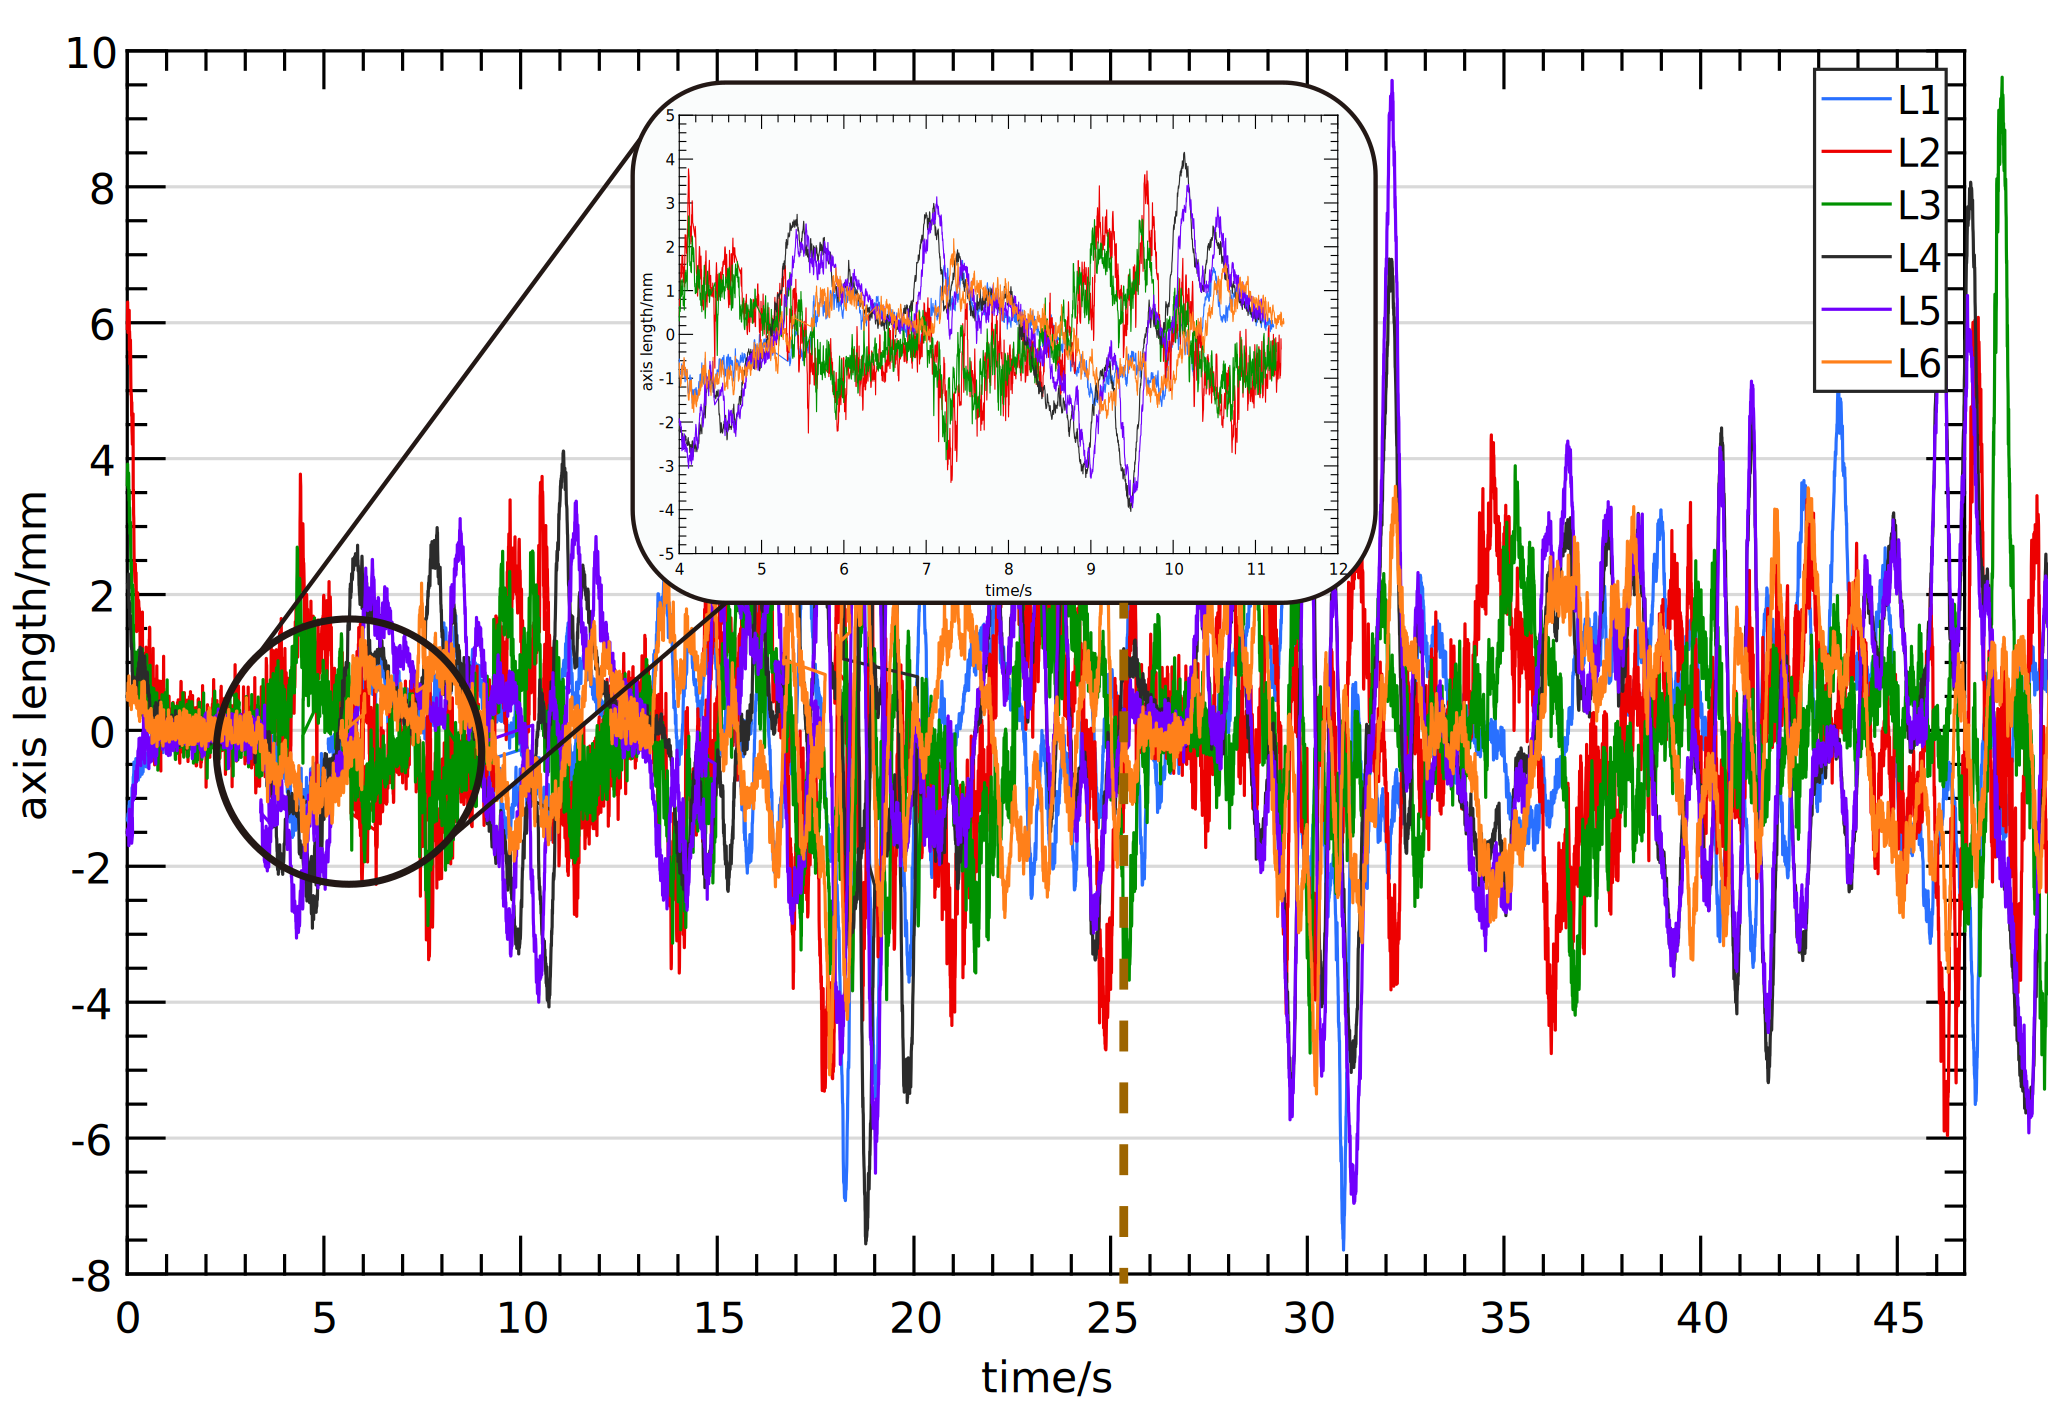
\includegraphics[width=0.6\textwidth]{imgs/Experiment/C-AL-FM_1_axis_diff_length.png}
    \caption{凸优化-自适应滑膜控制器在输入低振幅、高频率情况下的轴长跟踪误差}
    \label{fig:C-AL-FM_1_axis_diff_length}
\end{figure}

\begin{figure}[H]
    \centering
    \includegraphics[width=0.6\textwidth]{imgs/Experiment/C-AL-FM_1_c_movement.png}
    \caption{凸优化-自适应滑膜控制器在输入低振幅、高频率情况下,正解得到的C平台位置移动情况}
    \label{fig:C-AL-FM_1_c_movement}
\end{figure}

对比前面高振幅、低频率的情形,此时尽管输入的振幅减小为之前的一半左右,但其变化频率明显增大。在15s前,对应的轴的跟踪精度下降,每根轴误差被放大到
$\left[ -3\mathrm{mm},4\mathrm{mm} \right] $,而C平台的控制精度则降低到$\left[ -5\mathrm{mm},5\mathrm{mm} \right] $(x轴)。在15s后,y轴振动速度更快,此时轴的跟踪精度下降到$\left[ -6\mathrm{mm},6\mathrm{mm} \right] $,C平台的精度下降到$\left[ -10\mathrm{mm},10\mathrm{mm} \right] $,且可以发现,C平台在y轴方向振动很厉害。这表明控制器这样的高频下跟踪精度下降很快,同时凸优化规划器在这里也起了一定的作用,类似一个低通滤波器将轨迹平滑了。

对比PID控制器在高振幅、低频率下的控制情况,结果如图所示:

\begin{figure}[H]
    \centering
    \subfloat[输入扰动x,y,z三方向振幅]{
    \begin{minipage}[t]{0.4\linewidth}
    \centering
    \includegraphics[width=0.9\textwidth]{imgs/Experiment/P-AH-FL_1_position_B_error.png}
    % \caption{}
    \end{minipage}%
    }%
    \hspace{0.5pt}
    \subfloat[输入扰动RPY角振幅]{
    \begin{minipage}[t]{0.4\linewidth}
    \centering
    \includegraphics[width=0.9\textwidth]{imgs/Experiment/P-AH-FL_1_rpy_B.png}
    % \caption{}
    \end{minipage}%
    }%
    \centering
    \caption[]{PID控制器对应的输入扰动振幅}
    \label{fig:P-AH-FL_1_input}
\end{figure}

\begin{figure}[H]
    \centering
    \subfloat[6轴实际轴长]{
    \begin{minipage}[t]{0.4\linewidth}
    \centering
    \includegraphics[width=0.9\textwidth]{imgs/Experiment/P-AH-FL_1_axis_actual_length.png}
    % \caption{}
    \end{minipage}%
    }%
    \hspace{0.5pt}
    \subfloat[6轴期望轴长]{
    \begin{minipage}[t]{0.4\linewidth}
    \centering
    \includegraphics[width=0.9\textwidth]{imgs/Experiment/P-AH-FL_1_axis_ideal_length.png}
    % \caption{}
    \end{minipage}%
    }%
    \centering
    \caption[]{PID控制器在输入低振幅、高频率情况下的轴长响应图}
    \label{fig:P-AH-FL_1_axis}
\end{figure}

\begin{figure}[H]
    \centering
    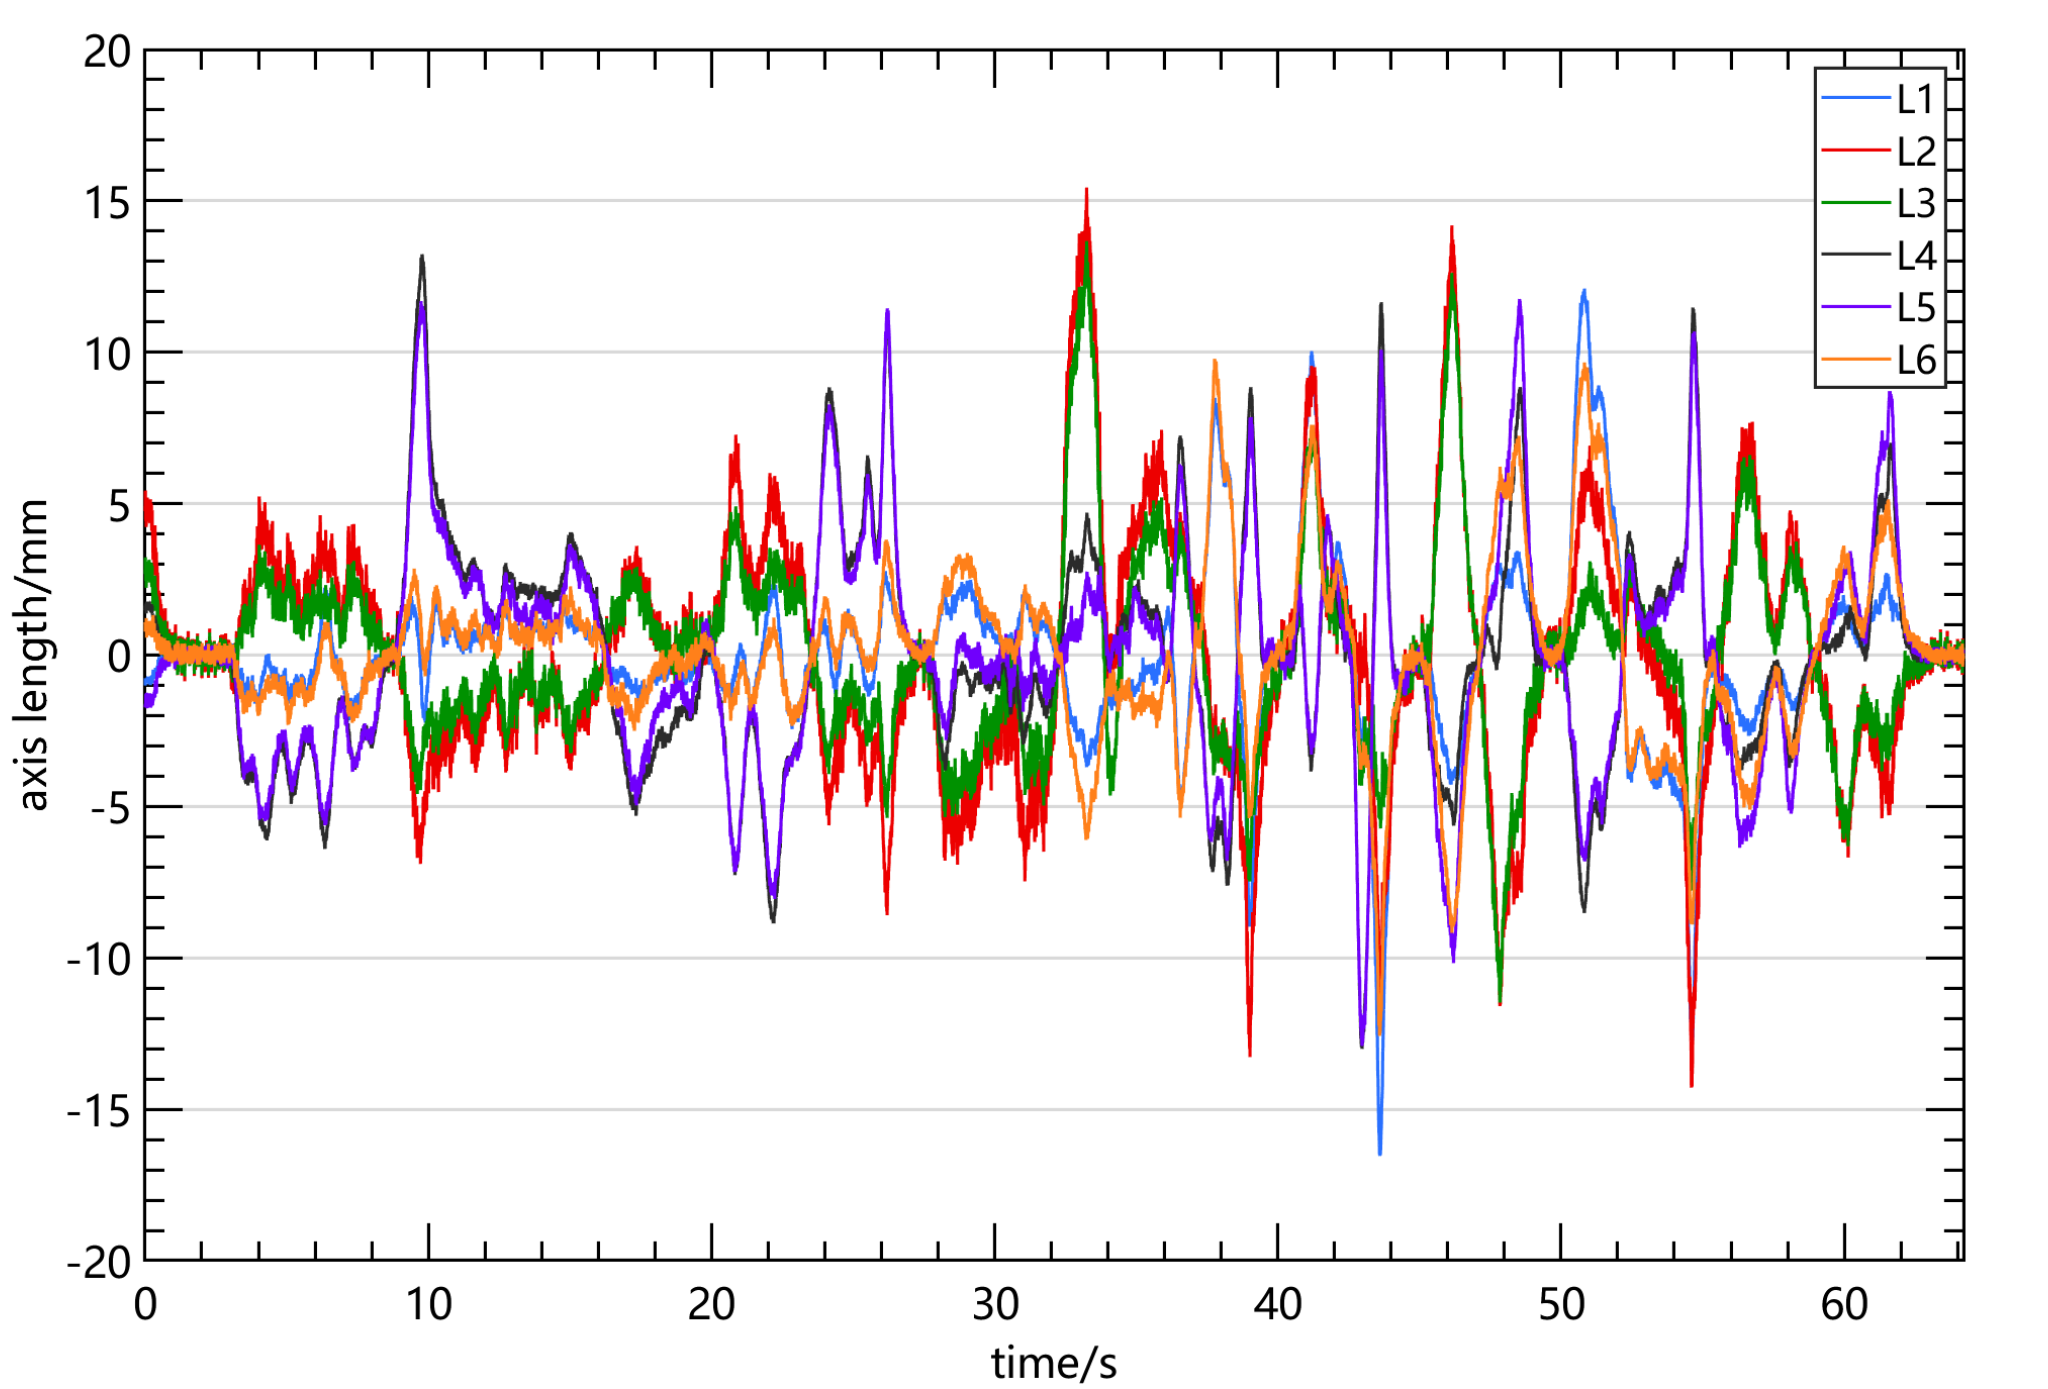
\includegraphics[width=0.6\textwidth]{imgs/Experiment/P-AH-FL_1_axis_diff_length.png}
    \caption{PID控制器在输入低振幅、高频率情况下的轴长跟踪误差}
    \label{fig:P-AH-FL_1_axis_diff_length}
\end{figure}

\begin{figure}[H]
    \centering
    \includegraphics[width=0.6\textwidth]{imgs/Experiment/P-AH-FL_1_c_movement.png}
    \caption{PID控制器在输入低振幅、高频率情况下,正解得到的C平台位置移动情况}
    \label{fig:P-AH-FL_1_c_movement}
\end{figure}

对比PID控制器和本文提出的滑膜控制器结果,可以发现,其轴的跟踪精度在$\left[ -6\mathrm{mm},10\mathrm{mm} \right] $
左右,对应的C平台位置精度为$x:\left[ -6\mathrm{mm},6\mathrm{mm} \right] ,y:\left[ -10\mathrm{mm},10\mathrm{mm} \right] $,其精度差于本文的控制器。

如果直接将逆解轴长作为控制量进行控制,其结果为:

\begin{figure}[H]
    \centering
    \subfloat[输入扰动x,y,z三方向振幅]{
    \begin{minipage}[t]{0.4\linewidth}
    \centering
    \includegraphics[width=0.9\textwidth]{imgs/Experiment/N-AH-FL_1_position_B_error.png}
    % \caption{}
    \end{minipage}%
    }%
    \hspace{0.5pt}
    \subfloat[输入扰动RPY角振幅]{
    \begin{minipage}[t]{0.4\linewidth}
    \centering
    \includegraphics[width=0.9\textwidth]{imgs/Experiment/N-AH-FL_1_rpy_B.png}
    % \caption{}
    \end{minipage}%
    }%
    \centering
    \caption[]{无控制器时的输入扰动振幅}
    \label{fig:N-AH-FL_1_input}
\end{figure}

\begin{figure}[H]
    \centering
    \subfloat[6轴实际轴长]{
    \begin{minipage}[t]{0.4\linewidth}
    \centering
    \includegraphics[width=0.9\textwidth]{imgs/Experiment/N-AH-FL_1_axis_actual_length.png}
    % \caption{}
    \end{minipage}%
    }%
    \hspace{0.5pt}
    \subfloat[6轴期望轴长]{
    \begin{minipage}[t]{0.4\linewidth}
    \centering
    \includegraphics[width=0.9\textwidth]{imgs/Experiment/N-AH-FL_1_axis_ideal_length.png}
    % \caption{}
    \end{minipage}%
    }%
    \centering
    \caption[]{无控制器时,输入低振幅、高频率情况下的轴长响应图}
    \label{fig:N-AH-FL_1_axis}
\end{figure}

\begin{figure}[H]
    \centering
    \includegraphics[width=0.6\textwidth]{imgs/Experiment/N-AH-FL_1_axis_diff_length.png}
    \caption{无控制器时,输入低振幅、高频率情况下的轴长跟踪误差}
    \label{fig:N-AH-FL_1_axis_diff_length}
\end{figure}

\begin{figure}[H]
    \centering
    \includegraphics[width=0.6\textwidth]{imgs/Experiment/N-AH-FL_1_c_movement.png}
    \caption{无控制器时,输入低振幅、高频率情况下,正解得到的C平台位置移动情况}
    \label{fig:N-AH-FL_1_c_movement}
\end{figure}

可以发现,直接将轴长作为控制量进行控制,最终轴的跟踪精度在$\left[ -6\mathrm{mm},10\mathrm{mm} \right] $左右,对应的C平台位置精度为$x:\left[ -15\mathrm{mm},15\mathrm{mm} \right] ,y:\left[ -5\mathrm{mm},10\mathrm{mm} \right] $,其精度比PID差一点。这是因为如果直接将轴长进行反馈,轴的运动会产生反作用力,改变B的位姿,从而使C的位姿发生变化。因为控制周期不能无限小,因此这样做会不断产生误差,甚至在一定频率下,由支链的反作用力作为驱动发生激振。

% todo: 列出结果的表格,作为结束

实验结果表明,本文提出的控制器对悬浮的Stewart机构在外力扰动下的振动抑制有一定的作用。在频率较低的情况下,可以将振幅抑制为$10\%$左右;而对频率高的情况下,控制器做了安全措施来限制输出速度,保证机构安全的同时也使得跟踪误差增大。实验结果也验证了仿真分析得到的控制算法特点:

\begin{enumerate}
    \item 控制器是基于无模型的控制
    \item 控制器对噪声鲁棒,抗干扰能力强
    \item 控制器输出受限,保证仪器安全
    \item 控制器收敛速度快
\end{enumerate}
\FloatBarrier
